\documentclass[11pt]{article}
\pagestyle{plain}

% \pgfplotsset{compat=1.18}
\usepackage[margin=1in]{geometry}
\usepackage{amsmath,amsfonts,amssymb,amsthm}
\usepackage[ruled,vlined,linesnumbered,commentsnumbered]{algorithm2e}
\SetKwInput{KwIn}{Input}
\SetKwInput{KwOut}{Output}
\SetKwInput{KwGlobal}{Global variable}
\SetKwInput{KwOracle}{Oracle}
\SetKwComment{Comment}{// }{}
\usepackage{graphicx}
\usepackage{enumerate}
\usepackage{bbm}
\usepackage{verbatim}
\usepackage{hyperref,color}
\usepackage[capitalize,nameinlink]{cleveref}
\usepackage[dvipsnames]{xcolor}
\hypersetup{
	colorlinks=true,
	pdfpagemode=UseNone,
	citecolor=OliveGreen,
	linkcolor=NavyBlue,
	urlcolor=Magenta,
	pdfstartview=FitW
}
\usepackage{appendix}
\usepackage{makecell}
\usepackage{tablefootnote}
\crefname{appsec}{Appendix}{Appendices}
\usepackage{tikz}
\usepackage{pgfplots}
\usepackage{xifthen}
\usepackage{subcaption}
\usepackage{hhline}
\usepackage{listings}

\theoremstyle{plain}
\newtheorem{theorem}{Theorem}[section]
\newtheorem{proposition}[theorem]{Proposition}
\newtheorem{lemma}[theorem]{Lemma}
\newtheorem{corollary}[theorem]{Corollary}
\newtheorem{conjecture}[theorem]{Conjecture}
\newtheorem{problem}[theorem]{Problem}
\newtheorem{claim}[theorem]{Claim}
\newtheorem{fact}[theorem]{Fact}

\theoremstyle{definition}
\newtheorem{definition}[theorem]{Definition}
\newtheorem{example}[theorem]{Example}
\newtheorem{observation}[theorem]{Observation}
\newtheorem{assumption}[theorem]{Assumption}
\newtheorem*{assumption*}{Assumption}
\newtheorem{condition}[theorem]{Condition}

\theoremstyle{remark}
\newtheorem{remark}[theorem]{Remark}

\crefname{lemma}{Lemma}{Lemmas}
\crefname{theorem}{Theorem}{Theorems}
\crefname{definition}{Definition}{Definitions}
\crefname{fact}{Fact}{Facts}
\crefname{claim}{Claim}{Claims}
\crefname{proposition}{Proposition}{Propositions}


\newcommand{\dif}{\,\mathrm{d}}
%\newcommand{\E}{\mathbb{E}}
%\newcommand{\Var}{\mathrm{Var}}
\newcommand{\Cov}{\mathrm{Cov}}
\newcommand{\MI}{\mathrm{I}}
%\newcommand{\Ent}{\mathrm{Ent}}
\newcommand{\ind}{\mathbbm{1}}
\newcommand{\allone}{\mathbf{1}}
\newcommand{\tr}{\mathrm{tr}}
\newcommand{\wt}{\mathrm{weight}}
\DeclareMathOperator*{\argmax}{arg\,max}
\newcommand{\norm}[1]{\left\lVert #1 \right\rVert}
\newcommand{\TV}[2]{\left\|#1 - #2\right\|_{\mathrm{TV}}}
\newcommand{\ceil}[1]{\left\lceil #1 \right\rceil}
\newcommand{\floor}[1]{\left\lfloor #1 \right\rfloor}
\newcommand{\ip}[2]{\left\langle #1 , #2 \right\rangle}
\newcommand{\grad}{\nabla}
\newcommand{\hessian}{\nabla^2}
\newcommand{\trans}{\intercal}
\newcommand{\diag}{\mathrm{diag}}
\newcommand{\poly}{\mathrm{poly}}
\newcommand{\dist}{\mathrm{dist}}
\newcommand{\sgn}{\mathrm{sgn}}
\newcommand{\fpras}{\mathsf{FPRAS}}
\newcommand{\fpaus}{\mathsf{FPAUS}}
\newcommand{\fptas}{\mathsf{FPTAS}}

\newcommand{\eps}{\varepsilon}

\newcommand{\N}{\mathbb{N}}
\newcommand{\Z}{\mathbb{Z}}
\newcommand{\Q}{\mathbb{Q}}
\newcommand{\R}{\mathbb{R}}
\newcommand{\C}{\mathbb{C}}

\renewcommand{\AA}{\mathcal{A}}
\newcommand{\BB}{\mathcal{B}}
\newcommand{\CC}{\mathcal{C}}
\newcommand{\DD}{\mathcal{D}}
\newcommand{\EE}{\mathcal{E}}
\newcommand{\FF}{\mathcal{F}}
\newcommand{\GG}{\mathcal{G}}
\newcommand{\HH}{\mathcal{H}}
\newcommand{\II}{\mathcal{I}}
\newcommand{\JJ}{\mathcal{J}}
\newcommand{\KK}{\mathcal{K}}
\newcommand{\LL}{\mathcal{L}}
\newcommand{\MM}{\mathcal{M}}
\newcommand{\NN}{\mathcal{N}}
\newcommand{\OO}{\mathcal{O}}
\newcommand{\PP}{\mathcal{P}}
\newcommand{\QQ}{\mathcal{Q}}
\newcommand{\RR}{\mathcal{R}}
\renewcommand{\SS}{\mathcal{S}}
\newcommand{\TT}{\mathcal{T}}
\newcommand{\UU}{\mathcal{U}}
\newcommand{\VV}{\mathcal{V}}
\newcommand{\WW}{\mathcal{W}}
\newcommand{\XX}{\mathcal{X}}
\newcommand{\YY}{\mathcal{Y}}
\newcommand{\ZZ}{\mathcal{Z}}

\newcommand{\KL}[2]{D_{\mathrm{KL}} \left( #1 \,\Vert\, #2 \right)}
\newcommand{\KLbig}[2]{D_{\mathrm{KL}} \left( #1 \,\big\Vert\, #2 \right)}
\newcommand{\KLBig}[2]{D_{\mathrm{KL}} \left( #1 \,\Big\Vert\, #2 \right)}

\newcommand{\SKL}[2]{D_{\mathrm{SKL}} \left( #1 \,\Vert\, #2 \right)}
\newcommand{\SKLbig}[2]{D_{\mathrm{SKL}} \left( #1 \,\big\Vert\, #2 \right)}
\newcommand{\SKLBig}[2]{D_{\mathrm{SKL}} \left( #1 \,\Big\Vert\, #2 \right)}

\newcommand{\qandq}{\quad\text{and}\quad}
\newcommand{\supp}{\mathrm{supp}}

\newcommand{\DKL}[2]{\-D_{\-{KL}}\left(#1 \parallel #2\right)}
\newcommand{\DTV}[2]{\-D_{\mathrm{TV}}\left({#1},{#2}\right)}
% \newcommand{\dist}{\mathrm{dist}}
\newcommand{\e}{\mathrm{e}}
\renewcommand{\epsilon}{\varepsilon}
\renewcommand{\emptyset}{\varnothing}
% \newcommand{\norm}[1]{\left\Vert#1\right\Vert}
\newcommand{\set}[1]{\left\{#1\right\}}
\newcommand{\tuple}[1]{\left(#1\right)} 
% \newcommand{\eps}{\varepsilon}
\newcommand{\inner}[2]{\left\langle #1,#2\right\rangle}
\newcommand{\tp}{\tuple}
\newcommand{\ol}{\overline}
\newcommand{\abs}[1]{\left\vert#1\right\vert}
\newcommand{\ctp}[1]{\left\lceil#1\right\rceil}
\newcommand{\ftp}[1]{\left\lfloor#1\right\rfloor}
\newcommand{\Ind}[1]{\-{Ind}_{#1}}
\newcommand{\todo}[1]{{\color{red} TODO: #1}}

\newcommand{\Cor}{\Psi^{\mathrm{sym}}}
\newcommand{\cor}{\Psi^{\-{cor}}}
\newcommand{\Inf}{\Psi}
% \newcommand{\diag}{\-{diag}}

\def\*#1{\boldsymbol{#1}} % Use \*A for \mathbf{A}
\def\+#1{\mathcal{#1}} % Use \+A for \mathcal{A}
\def\-#1{\mathrm{#1}} % Use \-A for \mathrm{A}
\def\=#1{\mathbb{#1}} % Use \^A for \mathbb{A}
\def\!#1{\mathfrak{#1}} % Use \!A for \mathfrak{A}

\newcommand*\diff{\mathop{}\!\mathrm{d}}

% probability
% \DeclareMathOperator*{\oPr}{\mathbf{Pr}}
\def\oPr{\mathop{\mathrm{Pr}}}
\renewcommand{\Pr}[2][]{ \ifthenelse{\isempty{#1}}
  {\oPr\left[#2\right]}
  {\oPr_{#1}\left[#2\right]} } % Use \Pr[a]{b} for \mathbf{Pr}_a[b], \Pr{b} for  \mathbf{Pr}[b]

% expectation: relies on the package "dsfont"
% \DeclareMathOperator*{\oE}{\mathbb{E}}
\def\oE{\mathop{\mathbb{E}}}
\newcommand{\E}[2][]{ \ifthenelse{\isempty{#1}}
  {\oE\left[#2\right]}
  {\oE_{#1}\left[#2\right]} }

% variance
%\DeclareMathOperator*{\oVar}{\mathbf{Var}}
\def\oVar{\mathrm{Var}}
\newcommand{\Var}[2][]{ \ifthenelse{\isempty{#1}}
  {\oVar\left[#2\right]}
  {\oVar_{#1}\left[#2\right]} }

% entropy
% \DeclareMathOperator*{\oEnt}{\mathbf{Ent}}
\def\oEnt{\mathrm{Ent}}
\newcommand{\Ent}[2][]{ \ifthenelse{\isempty{#1}}
  {\oEnt\left[#2\right]}
  {\oEnt_{#1}\left[#2\right]} }

\newcommand{\PhiEnt}[2][]{ \ifthenelse{\isempty{#1}}
  {\oEnt^\phi\left[#2\right]}
  {\oEnt^\phi_{#1}\left[#2\right]} }


\newenvironment{Exampleparagraph}[1][]
{
    \par 
    \noindent 
    \textbf{\color{blue} #1}
    \par 
    \vspace{0.5em} 
    \itshape 
}
{
    \par 
    \vspace{1em} 
}

%\input{local-macro}

\newcommand{\RED}[1]{\textcolor{red}{#1}}

\newcommand{\bern}[1]{\mathrm{Bern}\left(#1\right)}
\newcommand{\pll}{\parallel}



\title{CS 7545 F26, Computational Mini Project 3}
\date{Due on November 19, 2026}
\author{{\textbf{Zejia Chen}} \\ \textbf{GTID: 904178159}}

\pgfplotsset{compat=1.18} 
\begin{document}

\maketitle
\section*{Part 1}
\subsection*{Part 1.A}
The following are plots of $0$ or $3$ observations with length scale $0.2$.
\begin{figure}[htbp!]
    \centering
    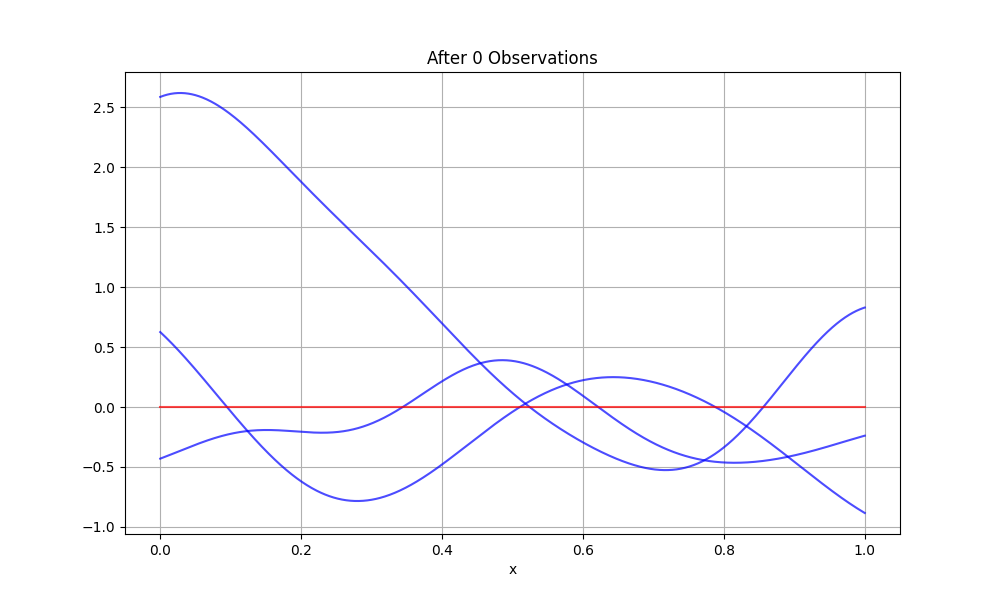
\includegraphics[width=0.47\linewidth]{pictures/Part 1.A/After 0 Observations.png}\hfill
    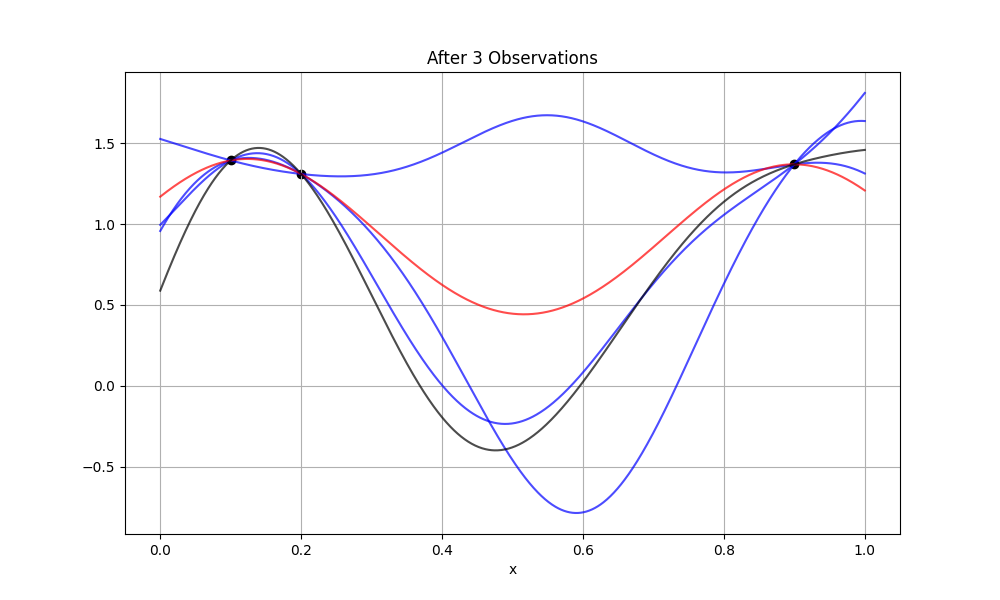
\includegraphics[width=0.47\linewidth]{pictures/Part 1.A/After 3 Observations.png}
    \caption{Results after 0 observations (left) and 3 observations (right) length scale 0.2.}
    \label{fig:part1A}
\end{figure}
\begin{itemize}
    \item [1.] All functions sampled from the posterior match the observations.
    \item [2.] The mean changed from a constant function to a curve that matches all the observations.
\end{itemize}
\subsection*{Part 1.B}
The following are plots of $0$ or $3$ observations with length scale $0.05$.
\begin{figure}[htbp!]
    \centering
    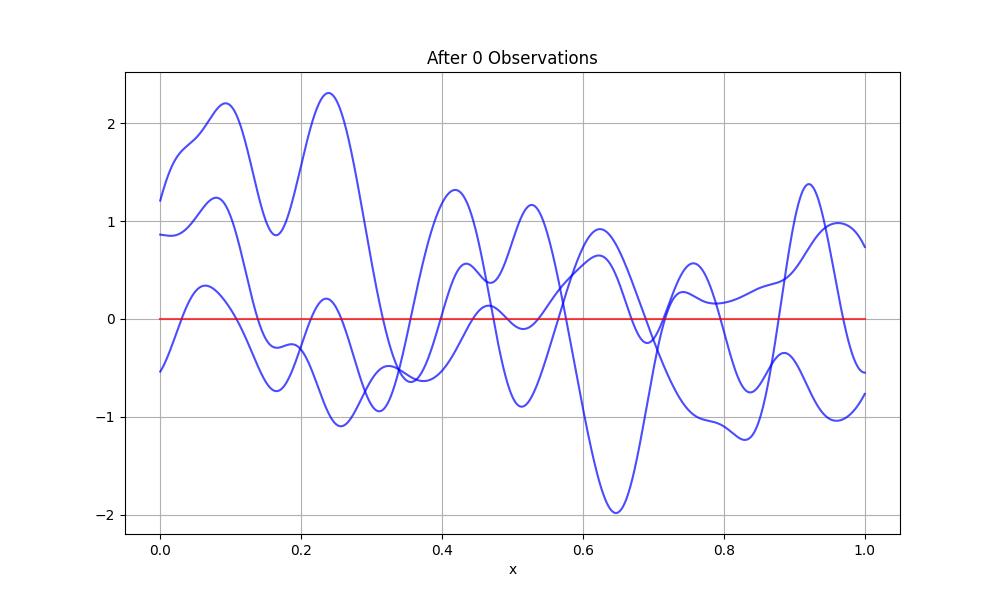
\includegraphics[width=0.47\linewidth]{pictures/Part 1.B/After 0 Observations.png}\hfill
    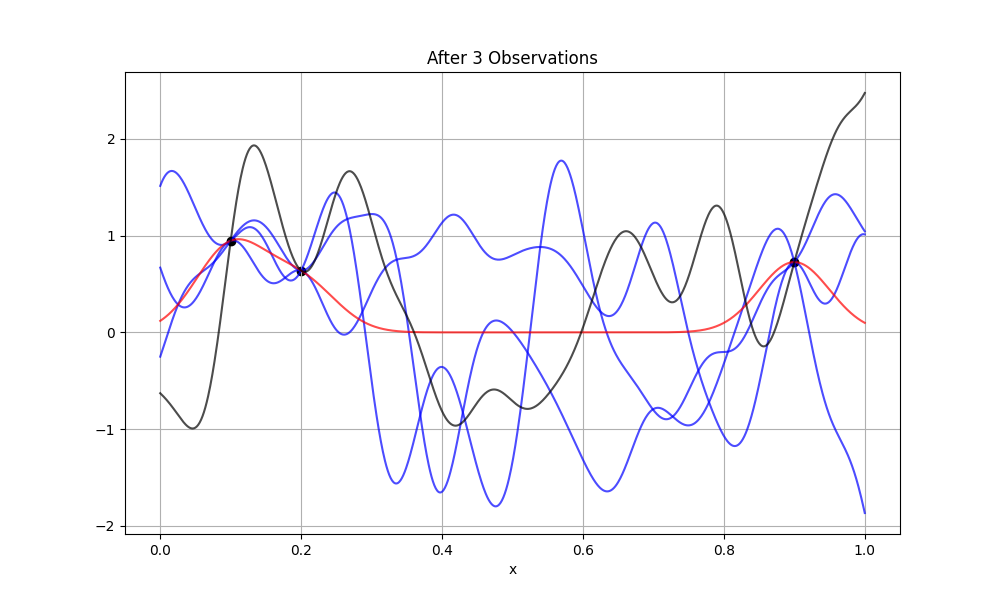
\includegraphics[width=0.47\linewidth]{pictures/Part 1.B/After 3 Observations.png}
    \caption{Results after 0 observations (left) and 3 observations (right) length scale 0.05.}
    \label{fig:part1B}
\end{figure}
\begin{itemize}
    \item [1.] The functions have more fluctuations and are more complicated than the functions sampled with length scale $0.2$.
    \item [2.] The observations only control a small neighbourhood of observed points for the mean function under the posterior distribution.
    The range of the ``neighbourhood'' depends on the length scale, which controls how quickly correlations decay with distance.
    With \(\ell=0.05\), the center of the interval is far from all observation locations relative to the length scale.
    Thus, its correlations with the observations are negligible, a posterior mean zero there.
\end{itemize}
\newpage\subsection*{Part 1.C}
The following are plots of eigenvalues and eigenvectors of the kernel matrix with length scale $0.2$ and $0.05$.
\begin{figure}[htbp!]
    \centering
    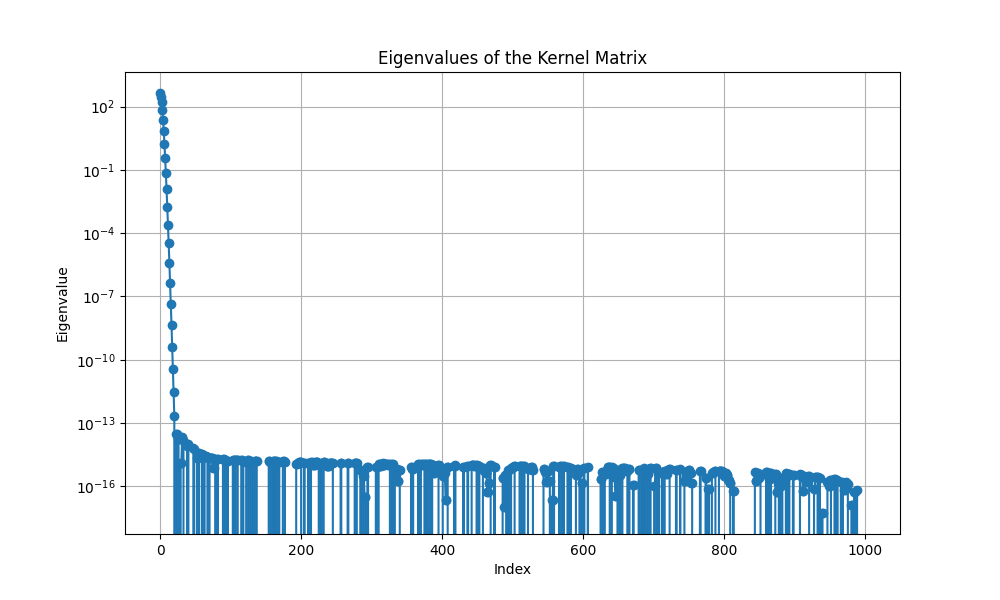
\includegraphics[width=0.47\linewidth]{pictures/Part 1.C/Eigenvalues_of_Kernel_Matrix_0.2.png}\hfill
    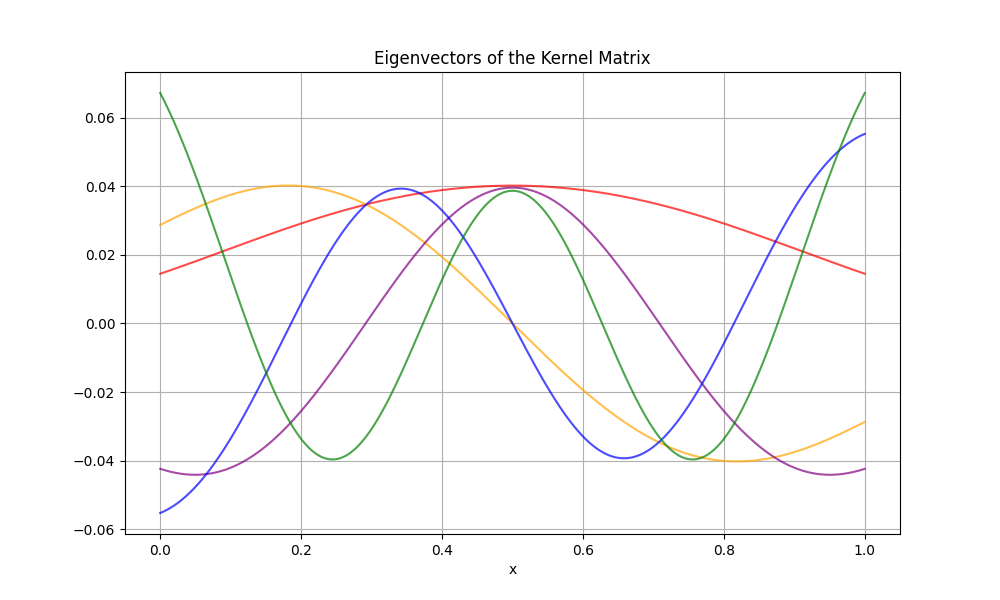
\includegraphics[width=0.47\linewidth]{pictures/Part 1.C/Eigenvectors of the Kernel Matrix_0.2.png}
    \caption{Eigenvalues and eigenvectors of the kernel matrix with length scale $0.2$.}
    \label{fig:part1C_0.2}
\end{figure}
\begin{figure}[htbp!]
    \centering
    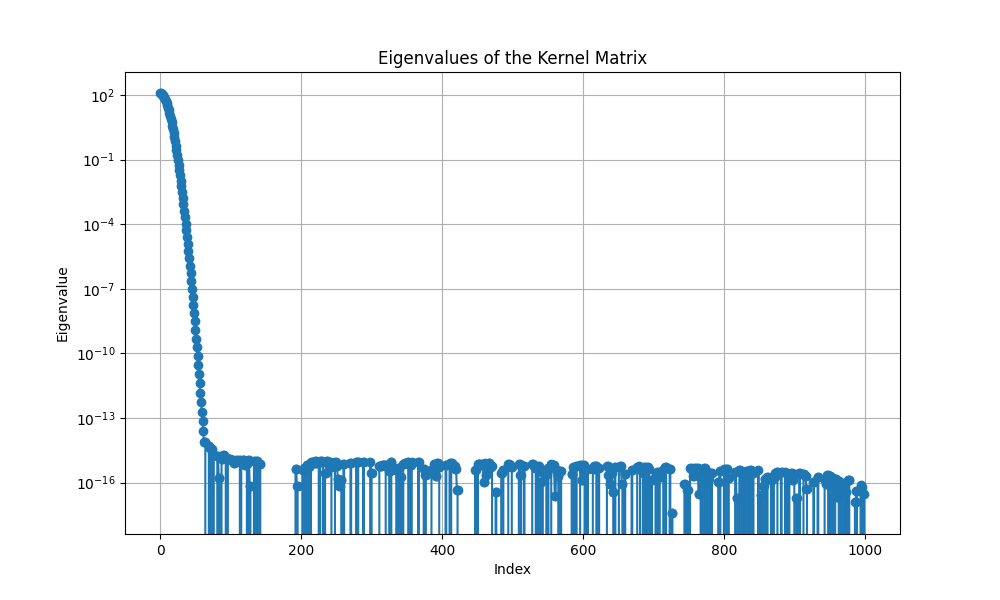
\includegraphics[width=0.47\linewidth]{pictures/Part 1.C/Eigenvalues_of_Kernel_Matrix_0.05.png}\hfill
    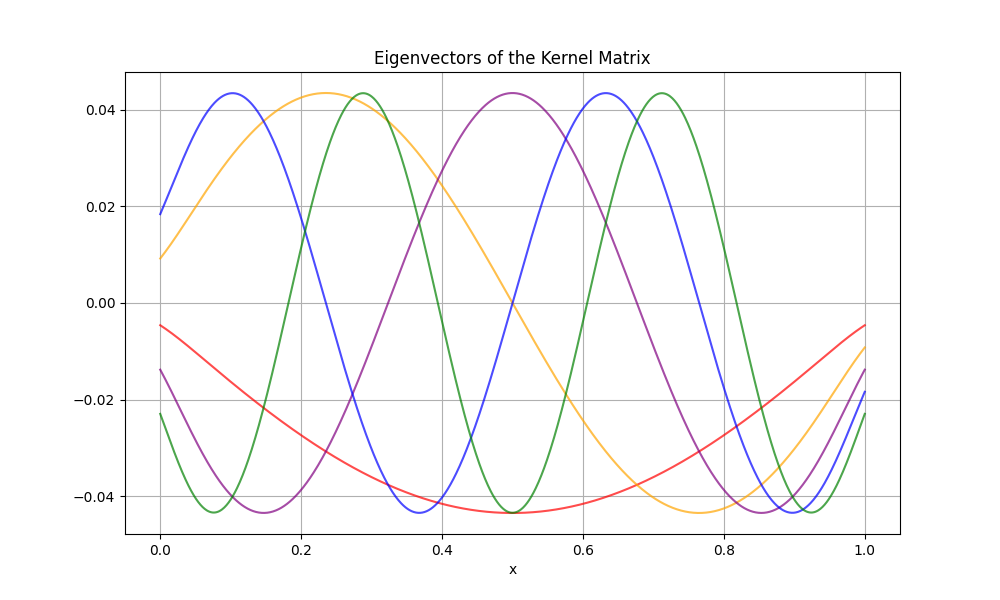
\includegraphics[width=0.47\linewidth]{pictures/Part 1.C/Eigenvectors of the Kernel Matrix_0.05.png}
    \caption{Eigenvalues and eigenvectors of the kernel matrix with length scale $0.05$.}
    \label{fig:part1C_0.05}
\end{figure}
\begin{itemize}
    \item [1.] For eigenvalue spectra, the eigenvalues decay faster for \(\ell=0.2\), and therefore, more variance is concentrated in the leading eigenfunctions.
    
    The sampled function is a linear combination of eigenfunctions with respect to eigenvalues.
    For $\ell = 0.2$, the eigenvalues are more concentrated on the leading ones, therefore, the sampled function will be more concentrated on the small portion of eigenfunctions with large eigenvalues.
    This means that the one with larger scale has fewer fluctuations than the one with smaller scale.

    \item [2.] All the eigenfunctions are in the shape of $\sin$ function.
    The eigenfunctions appear to oscillate more rapidly for the smaller length scale and have more similar peak magnitudes than those for the larger length scale.
\end{itemize}

\section*{Part 2}
\subsection*{Part 2.A}
\begin{figure}[htbp!]
    \centering
    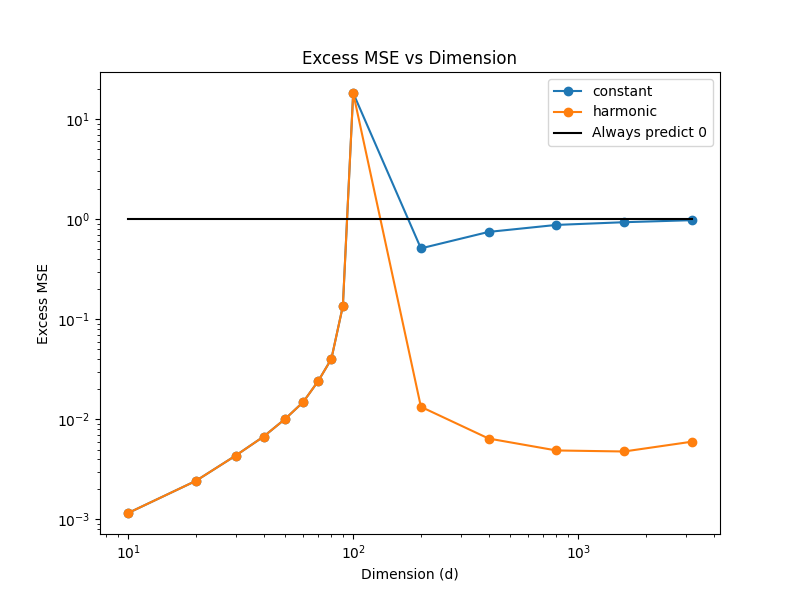
\includegraphics[width=0.7\linewidth]{pictures/Part 2/excess_mse_vary_eigs_constant_harmonic.png}
    \caption{Plot of excess MSE for constant and harmonic eigenvalue spectra.}
    \label{fig:part2A}
\end{figure}
\begin{itemize}
    \item [1.] When $n=d$, the excess MSEs are the same for the constant eigenvalue spectrum and the harmonic spectrum and among all the dimensions, it has the largest error.
    \item [2.] When $d < n$, the excess MSEs for two spectra are the same and increasing with respect to $d$.
    \item [3.] When $d > n$, the excess MSEs are first decreasing then increasing and they have a sharp drop near $d = n$.
    For the increasing period, the constant-spectrum excess MSE gradually approaches to $1$ but harmonic-spectrum excess MSE just increases very slightly.
    And the excess MSE for harmonic spectrum are much smaller than that one for constant spectrum. 
\end{itemize}
\newpage
\subsection*{Part 2.B}
\begin{figure}[htbp!]
    \centering
    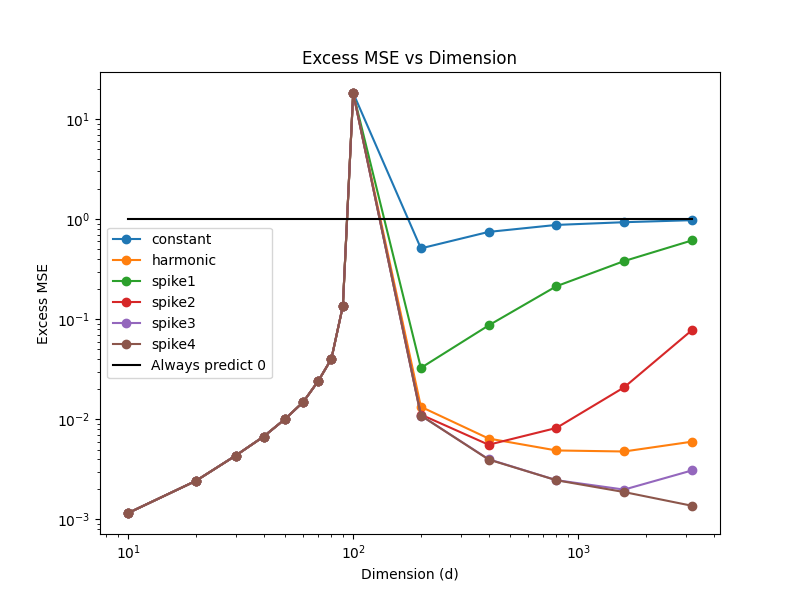
\includegraphics[width=0.6\linewidth]{pictures/Part 2/excess_mse_vary_eigs_spike.png}
    \caption{Plot of excess MSE for spiked eigenvalue spectra.}
    \label{fig:part2B}
\end{figure}
\begin{itemize}
    \item [1.] When $d > n$, most of excess MSEs are first decreasing then increasing, except spike4, which only decreases throughout the tested range.
    They all have a sharp drop near $d=n$.
    \item [2.] Smaller $\eps$ gives lower excess MSE and shifts the minimizer toward larger dimensions.
\end{itemize}
\subsection*{Part 2.C}
\begin{figure}[htbp!]
    \centering
    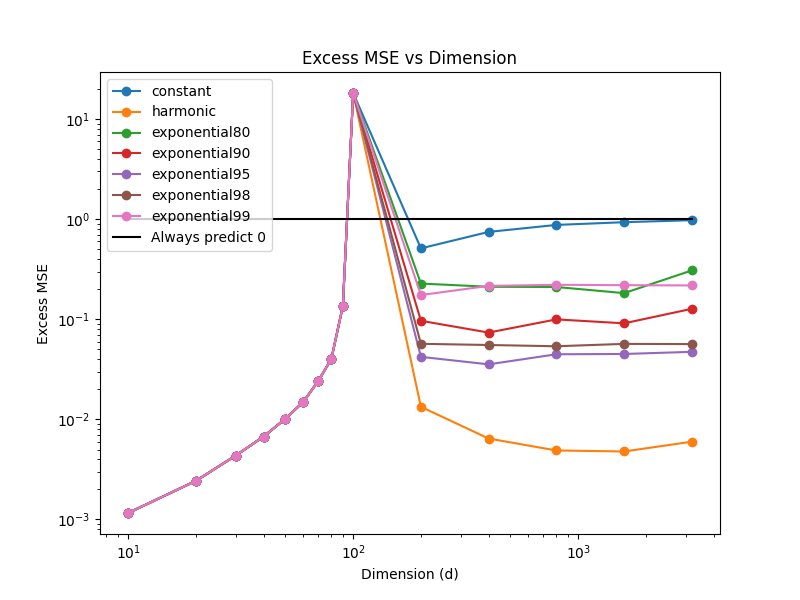
\includegraphics[width=0.6\linewidth]{pictures/Part 2/excess_mse_vary_eigs_exp.png}
    \caption{Plot of excess MSE for exponential eigenvalue spectra.}
    \label{fig:part2C}
\end{figure}
\begin{itemize}
    \item [1.] After dropping sharply from the peak near $d=n$, the excess MSE remains almost unchanged with some fluctuations across the tested dimensions.
    \item [2.] For $d > n$, the excess MSE generally decreases as $r$ increases from $0.8$ to $0.95$, then increases as $r$ increases to $0.99$.
\end{itemize}
\subsection*{Part 2.D}
\begin{figure}[htbp!]
    \centering
    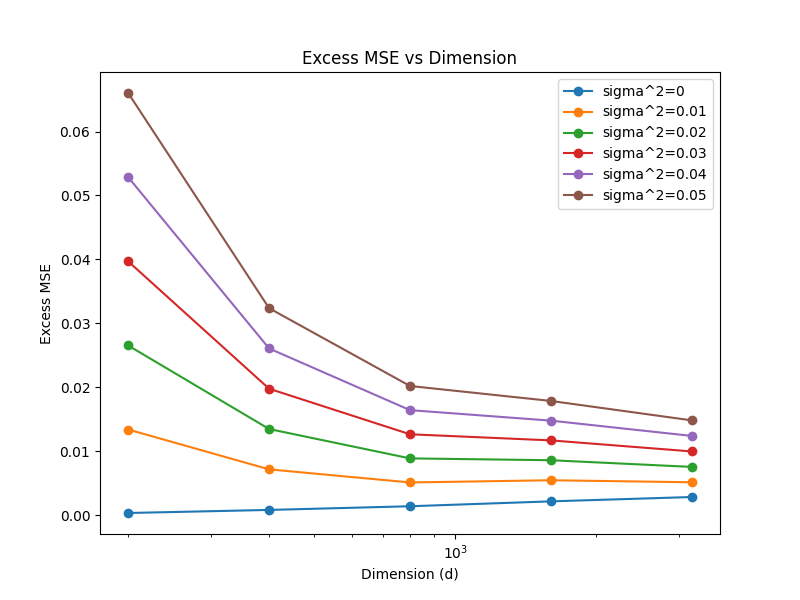
\includegraphics[width=0.7\linewidth]{pictures/Part 2/excess_mse_vary_sigma.png}
    \caption{Plot of excess MSE varying with $\sigma^2$.}
    \label{fig:part2D}
\end{figure}

By the expected excess MSE equation, we have that
$$
\E[y]{L(\hat\theta)-L(\theta^\star)\mid X} =
(\theta^\star)^\top B\theta^\star
+\sigma^2\operatorname{Tr}(C).
$$
where $B$ and $C$ only depend on the data $\{x_i\}_{i\in[n]}$.
See \emph{lecture notes 10} for formal definitions.
By concentration phenomenon, the excess MSE will be concentrated near its expectation with high probability.
This implies that for fixed dimension, the excess MSE will increase almost linearly in $\sigma^2$, which matches the ordering of the curves. 

Fix $\sigma^2$. 
For the harmonic spectrum over the tested dimensions, the bias contribution $(\theta^\star)^\top B\theta^\star$ increases with \(d\), while the variance contribution $\sigma^2\operatorname{Tr}(C)$ decreases.
If $\sigma^2 = 0$, only the bias contribution remains, giving the increasing curve.
If $\sigma^2 > 0$, the excess MSE generally decreases since the variance contribution usually dominates the bias contribution.

\end{document}